\chapter{\textbf{Revisão de Literatura}}\label{cap:revisao_de_literatura}

    \section{Parâmetros Estelares}
   		A compreensão dos parâmetros fotométricos e espectroscópicos é fundamental para a caracterização detalhada das estrelas. A integração desses dois conjuntos de dados possibilita uma visão abrangente das propriedades físicas e dinâmicas das estrelas, facilitando a classificação estelar, a identificação de estágios evolutivos e a investigação de fenômenos astrofísicos complexos. Nesta seção, será realizada uma revisão teórica dos principais parâmetros envolvidos no estudo abordado neste trabalho.

        A magnitude e o índice de cor das estrelas são conceitos fundamentais na astronomia para medir e descrever o brilho e as propriedades espectrais das estrelas. A magnitude (\(\lambda\)) é uma medida do brilho de uma estrela e está relacionado ao logaritmo do fluxo observado (\textit{F}), como descrito na equação (\ref{eq:mag}) em termos de uma constante de proporcionalidade (\(\beta\)), \cite{thanu_2006}.
        
        \begin{equation}\label{eq:mag}
        	\lambda = \beta - 2,5 \log F
        \end{equation}
    
         A magnitude absoluta (\(\Lambda\)) é uma medida padrão do brilho de uma estrela a uma distância de 10 parsecs\footnote{ 1 parsec equivale à aproximadamente \(3,0857\times10^{16}\) m} da Terra, segundo a equação (\ref{eq:absmag}) abaixo:
        
        \begin{equation}
        	\label{eq:absmag}
        	\Lambda = -5 ~\log_{10}(d) + 5 + \lambda
        \end{equation}
        
        Aqui, \(d\) é a distância ao aglomerado. Da maneira como foi definida, quanto mais brilhante é um objeto, menor será sua magnitude. 
         
        
        \begin{figure}[!h]
        	\centering
        	\caption[Curvas de transmissão dos filtros  no sistema Johson.]{Curvas de transmissão dos filtros no sistema Johson.}
        	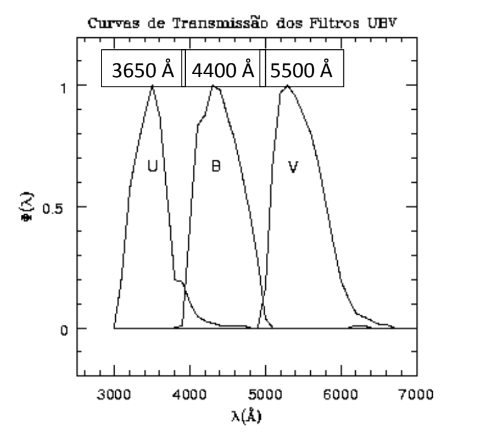
\includegraphics[width=0.5\linewidth]{04-figuras/ubv.png}\\
        	Fonte: https://www.if.ufrgs.br/tex/fis02001/aulas/Aula15-122.pdf
        	\label{fig:filtros}
        \end{figure}
        
        Uma estrela emite radiação em diferentes comprimentos de onda e definem-se sistemas de magnitude que possuem filtros em diferentes bandas. Um sistema de magnitudes é definido pela sua eficiência \(\phi(\lambda)\) e por uma constante que define o ponto zero da escala. O sistema apresentado nessa figura é o sistema UBV, desenvolvido por Harold Lester Johnson (1921-1980) e William Wilson Morgan (1906-1994) em 1951. U, B e V indicam as magnitudes aparentes nas bandas espectrais ultravioleta, azul e amarelo, respectivamente, e têm seus comprimentos de onda efetivos em 3650 \AA, 4400 \AA \, e 5500 \AA. Um sistema muito utilizado é o sistema fotométrico de Johnson que pode ser visto na Figura \ref{fig:filtros}. Define-se a magnitude bolométrica, que é uma medida do brilho total da estrela, integrando sobre todas as frequências. O índice de cor da estrela é um conceito que se refere à diferença de magnitude em duas faixas de frequência, que pode ser expressa pela comparação entre o fluxo eletromagnético em cada uma das bandas segundo a equação (\ref{eq:ind_cor}).
        
        \begin{equation}\label{eq:ind_cor}
        	\lambda_a-\lambda_b = -2,5\log\left(\frac{F_{\lambda_a}}{F_{\lambda_b}}\right)
        \end{equation}
    
   		Por exemplo, o índice de cor B-V é a diferença entre a magnitude no filtro azul (B) e no filtro amarelo (V). Esta diferença fornece informações sobre a classificação espectral da estrela e sobre a sua temperatura superficial. Estrelas com índice B-V mais baixo são mais quentes e azuis, e estrelas com  índice B-V mais alto são mais frias e vermelhas. O brilho e o índice de cor são, portanto, ferramentas essenciais para a caracterização e estudo de estrelas, permitindo aos astrônomos inferir importantes propriedades físicas e evolutivas  das estrelas a partir de  observações de brilho e espectros, \cite{thanu_2006}.
        
        Quando um objeto astronômico emite radiação eletromagnética, as nuvens de gás e poeira no meio interestelar entre o objeto emissor e o observador podem absorver e dispersar parte dessa radiação. Segundo \citeonline{hartmann2008accretion}, o fenômeno do avermelhamento ocorre porque essa absorção e dispersão são mais intensas para comprimentos de onda mais curtos (azuis), resultando na observação do objeto com características alteradas, particularmente com um deslocamento da radiação para comprimentos de onda mais longos (vermelhos).
        
        \begin{figure}[!h]
        	\centering
        	\caption[Ilustração da extinção interestelar e avermelhamento.]{Ilustração do fenômeno conhecido como extinção (escurecimento) e avermelhamento (desvio para comprimentos de onda vermelhos). Quando a luz de uma estrela viaja através do espaço interestelar, encontra poeira e gás no meio interestelar. Esta poeira dispersa e absorve parte da luz, particularmente mais dos comprimentos de onda azuis. O observador percebe que a estrela é mais fraca e mais vermelha do que seria sem a poeira.}
        	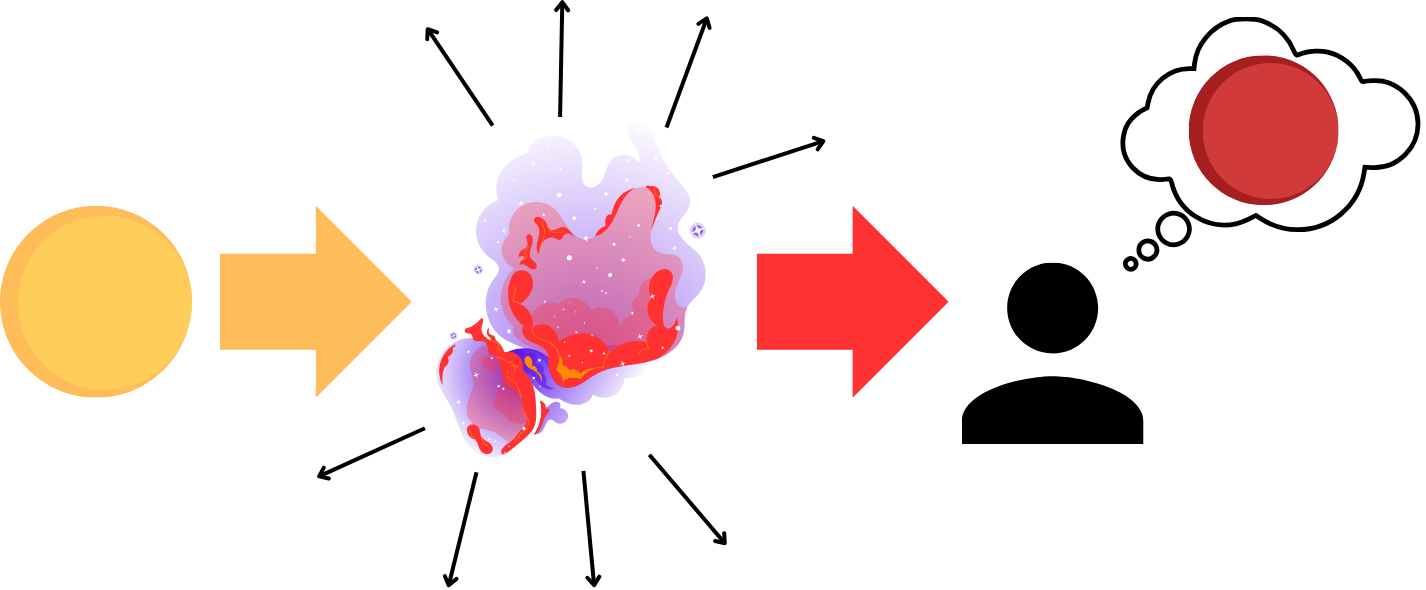
\includegraphics[width=0.5\linewidth]{04-figuras/extincao.png}\\
        	Fonte: Elaboração Própria. 
        	\label{fig:extinção}
        \end{figure}
        
        
        Na astronomia, o avermelhamento está diretamente associado à extinção interestelar, definida pela diferença entre o índice de cor observado e o índice de cor intrínseco, medindo o quanto a radiação foi deslocada para comprimentos de onda maiores.
        
        O conhecimento acerca do índice de cor intrínseco das estrelas é um elemento essencial no estudo das populações de estelares jovens. Não podemos assumir avermelhamento e extinção desprezáveis para a maioria das estrelas na pré-sequência principal (PMS, \textit{Pre-main-sequence}). O avermelhamento interestelar é convencionalmente estimado usando cores intrínsecas tabeladas para estrelas de campo anãs na sequência principal\footnote{ A sequência principal aparece como uma faixa contínua e distinta em um gráfico de índice de cor versus brilho das estrelas. As estrelas da sequência principal fundem átomos de hidrogênio para formar átomos de hélio em seus núcleos.} (MS) permitindo, assim, corrigir as magnitudes conforme descrito na equação (\ref{eq:bolmag}):
        
        \begin{equation}
        	\label{eq:bolmag}
        	\Lambda_{bol} =  \Lambda - A_\lambda + BC_\lambda \, ,
        \end{equation}
    	\noindent onde \(A_\lambda\) é o termo de correção relacionado ao avermelhamento e \(BC_\lambda\) o termo de correção bolométrico, a fim de obter o brilho total da estrela.
        
        A luminosidade representa a quantidade de energia eletromagnética irradiada por uma estrela, galáxia ou outro objeto astronômico por unidade de tempo. Junto com a temperatura efetiva, a luminosidade fornece pistas importantes sobre os estados evolutivos das estrelas. Podemos determinar a luminosidade a partir de fluxos corrigidos para os efeitos de escurecimento e avermelhamento de poeira no meio interestelar, entre o objeto astronômico e o observador,  \cite{hartmann2008accretion}.
        
        O gráfico da Figura \ref{fig:teff_spt} mostra a força das linhas espectrais de elementos químicos como He\(^+\), He, H, Ca\(^+\), Fe\(^+\) e TiO em função da temperatura estelar (3000 K a 50.000 K), correlacionado com os tipos espectrais (O5 a M0). A interpretação das linhas espectrais ajuda a distinguir temperaturas semelhantes: a presença de He\(^+\) indica temperaturas quentes, enquanto a presença de Ca\(^+\) e ausência de He\(^+\) aponta para temperaturas moderadas.
       
        
        \begin{figure}[!h]
        	\centering
        	\caption[Força de linhas espectrais de elementos químicos em função da temperatura.]{Intensidade de linhas espectrais como função da temperatura. Cortesia de Nick Strobel (https://www.astronomynotes.com/).}
        	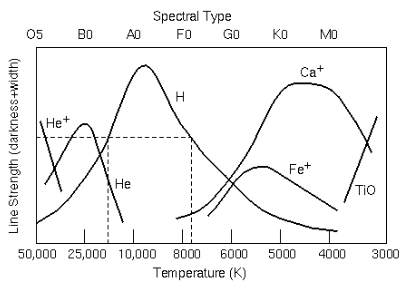
\includegraphics[width=0.5\linewidth]{04-figuras/linestr.png}\\
        	Fonte: \url{https://www.astronomynotes.com/starprop/s12.htm}. 
        	\label{fig:teff_spt}
        \end{figure}
        
		A classificação espectral é uma técnica fundamental e envolve a categorização de estrelas com base nos seus espectros. Ela revela informações sobre a temperatura, luminosidade, composição química e outras propriedades de uma estrela. O sistema mais amplamente utilizado para essa finalidade é o sistema MK (Morgan-Keenan), que classifica as estrelas utilizando classes de temperatura e classes de luminosidade, fornecendo uma estrutura abrangente para entender as características estelares. Gigantes Vermelhas (evoluídas) dividem a mesma classe de luminosidade de estrelas PMS, então a classe de luminosidade não determina absolutamente o estágio evolutivo.
        A força do sistema MK reside em sua capacidade de categorizar estrelas com base em características espectrais que indicam temperatura e gravidade superficial. Essa abordagem dupla permite uma compreensão mais detalhada das propriedades estelares e de seus estágios evolutivos. O sistema foi expandido para incluir uma ampla gama de tipos estelares, desde as estrelas mais quentes do tipo O até as anãs do tipo M mais frias, sendo adaptado para diferentes regiões do espectro, como o ultravioleta e o infravermelho, \cite{gray2009stellar}. A classificação das estrelas mais frias inclui a introdução de duas novas classes espectrais, L e T, identificadas através de dados do 2-Micron All-Sky Survey (2MASS). A classe L é definida para objetos mais frios do que as anãs M tardias, com temperaturas da ordem de 1500 a 2000 K, enquanto a classe T, exemplificada pelo objeto Gl 229B, apresenta um espetro dominado por metano, indicando temperaturas ainda mais baixas e o aparecimento de bandas de absorção molecular mais típicas de atmosferas planetárias, \cite{Kirkpatrick1999}.
		
		No diagrama de Hertzsprung-Russell (HRD, Figura \ref{fig:hrd}), a posição de uma estrela está correlacionada com seus parâmetros físicos, como luminosidade, temperatura efetiva, tipo espectral e raio estelar. Estrelas que ocupam a região diagonal do diagrama estão na sequência principal. A evolução das estrelas pode ser investigada com base na sua posição no HRD.
		
		\begin{figure}[!h]
			\centering
			\caption[Diagrama Hertzsprung-Russel]{O diagrama Hertzsprung-Russel para 22.000 estrelas do Catálogo Hipparcos \cite{ESA1997} e 1.000 anãs vermelhas e brancas do Catálogo Gliese \cite{Gliese1969}, destacando a Sequência Principal, onde estrelas como o Sol se situam, entre o canto superior esquerdo e o inferior direito.}
			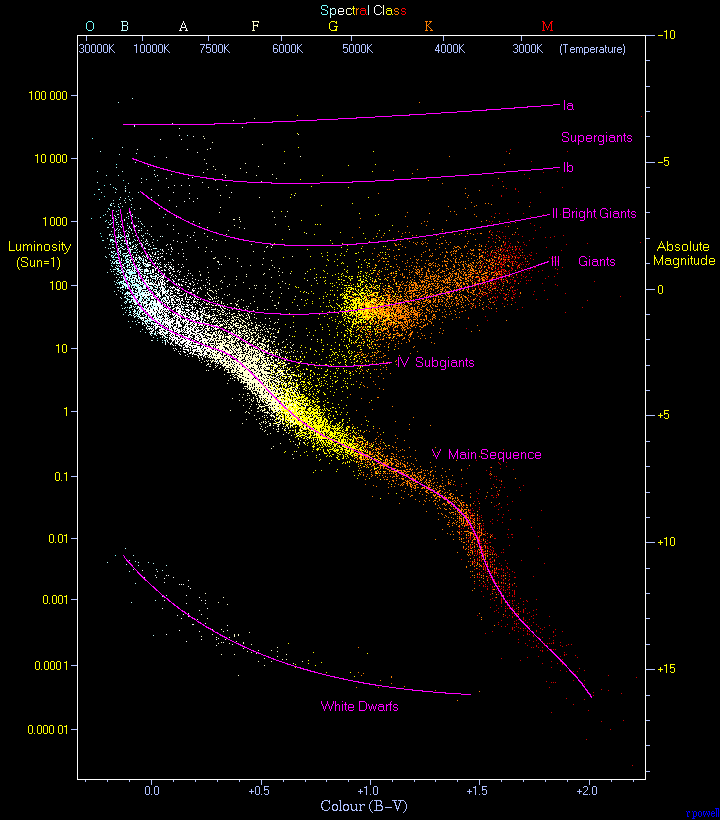
\includegraphics[width=0.5\linewidth]{04-figuras/HRDiagram.png}\\
			Fonte: http://www.atlasoftheuniverse.com/hr.html
			\label{fig:hrd}
		\end{figure}
	
	      No HRD, as estrelas jovens estão localizadas acima da sequência principal, na classe das Gigantes. Sua fonte de energia vem principalmente da contração gravitacional, com alguma contribuição da fusão de deutério em seu interior. Segundo \citeonline{hartmann2008accretion}, as estrelas jovens de baixa massa foram inicialmente identificadas como um subconjunto de objetos com linhas de emissão, normalmente exibindo forte emissão de linhas de hidrogênio (por exemplo H\(_\alpha\)), estando concentradas perto de associações de estrelas massivas (OB) e de nuvens moleculares. 
    
    \section{Massa Estelar}\label{sec:massa}
        A massa estelar é crucial para a física estelar. Vários processos, como a ocorrência de núcleos convectivos na sequência principal e a ignição da queima de hélio sob condições degeneradas ou não degeneradas, dependem do valor da massa da estrela, além da sua relação com outros parâmetros permitir obter informações que são de grande importância para compreensão de diversos campos da astrofísica estelar e galáctica.
        
        Segundo \citeonline{serenelli2021weighing}, a determinação precisa das massas estelares aprimora os modelos estelares, a determinação de distâncias no Universo, previsões de idade, taxas de acresção e de rotação de estrelas, além de leis de enriquecimento químico de galáxias.
        
        Para estrelas que fazem parte de sistemas binários, pode-se determinar a massa do par diretamente, utilizando a Terceira Lei de Kepler. Dessa forma, relações teóricas entre massa e parâmetros estelares como luminosidade e raio são comumente calculados a partir de sistemas binários de estrelas, como realizado em \citeonline{delfosse2000accurate} e \citeonline{chabrier2005initial}, sendo fundamentais para os modelos de evolução estelar, pois fornecem uma base observacional que permite inferir massas estelares a partir de características observáveis, como a magnitude e, a partir desta, a luminosidade. Os dados precisos de massa obtidos possibilitam a criação de relações que podem ser usadas para verificar a precisão de modelos teóricos, contribuindo para a calibração e melhoria dos modelos utilizados.
        
        Para a estimar ou determinar a massa individual de estrelas que não fazem parte de sistemas binários, há uma diversidade de métodos disponíveis. Para a sequência principal, a forma mais simples de se estimar a massa é usando as relações massa-luminosidade (M-L), citadas no parágrafo anterior, ou obtidas a partir de modelos de evolução estelar. Essas relações podem ser expressas como,
        
        \begin{equation}
			\label{eq:massai}
			M^* =  \beta L^\alpha
		\end{equation}
		ou,
		\begin{equation}
			\label{eq:massa1}
			\log(M^*) =  \alpha \log(L) + \log(\beta)
		\end{equation}
        
        Em \citeonline{serenelli2021weighing} os principais métodos são elencados e ranqueados conforme sua precisão. Aqueles empregados nesse trabalho pertencem à categoria de métodos dependentes de modelos teóricos\footnote{ São eles a relação massa-luminosidade ou massa-magnitude e o ajuste de isócronas}.
        De um lado, temos aqueles que aplicaram abordagens mais gerais do ajuste de isócronas, como os trabalhos de  \citeonline{jorgensen2005stellar}, \citeonline{kerber2005physical}, \citeonline{davies2014accretion} e \citeonline{dias2014self}. Em contrapartida, alguns estudos exploraram o método semi-empírico baseado na relação entre massa e luminosidade, como em \citeonline{delfosse2000accurate}, \citeonline{benedict2016solar}, 
        \citeonline{mann2019constrain},  \citeonline{giovinazzi2022mass} e  \citeonline{nidhi2023stellar}. Por fim, \citeonline{kerber2007physical} e \citeonline{kounkel2022untangling} adaptaram essa abordagem semi-empírica para um método fundamentado em modelos teóricos, utilizando dados de estrelas sintéticas, geradas a partir desses modelos teóricos, e obtendo relações para determinação de diversos parâmetros estelares. Essas distinções metodológicas refletem diferentes estratégias para estudar a determinação da massa.
        
    
    \section{Aprendizagem de Máquina}
        O advento recente de métodos de aprendizagem de máquina (\textit{Machine Learning}, ML) proporcionou ferramentas poderosas para prever resultados por meio do aprendizado de um conjunto de dados de entrada. Neste trabalho, os algoritmos de regressão analisam as relações entre os dados de um modelo teórico de evolução estelar, permitindo a previsão de valores para dados novos ou checagem da qualidade dos modelos pré-existentes. As técnicas populares incluem a regressão linear, árvores de decisão (e sua complexificação, bosques aleatórios) e redes neurais.  
        
        Na astrofísica, os modelos de regressão fundamentados no aprendizado de máquina são cada vez mais utilizados para determinar e estimar parâmetros estelares, como temperatura, luminosidade, composição química e massa, como realizado em  \citeonline{meingast2017estimating}, \citeonline{sarro2018estimates},
        \citeonline{wadekar2022sz}, \citeonline{kaeufer2023analysing}  e \citeonline{bello2023carmenes}. Ao analisar dados teóricos, pode-se construir um modelo particular para a determinação de um certo parâmetro ou para um conjunto de parâmetros.
    
